\setchapterpreamble[o]{%
  \dictum[Steve Jobs]{\textit{``Design is not  just what it looks like and
      feels like. Design is how it works.''}}}

\chapter{Design and Implementation}
\label{cha:design}

This chapter is about the design and implementation of the \emph{Xen-based
  Execution  Environment} (\gls{glo:XenBEE}).   The  execution environment
incorporates  a total  of three  main  components: the  \emph{xbe} on  the
user's side, the \emph{xbed} on  the server's side and the \emph{xbeinstd}
on  the  side of  a  single virtual  machine.   All  components have  been
implemented     using    the     \emph{Python}     programming    language
\cite{python-language}. In particular, version  $2.5$ of that language has
been used.

Some additional  modules and programs, that  are not part  of the standard
libraries shipped with Python, have been used, though. Among these are for
instance  the \texttt{twisted}  framework \cite{twisted-python}  which has
been  used  for  the  network  code,  a  library  called  \texttt{libvirt}
\cite{libvirt}  that  was used  to  connect  to  the Xen  virtual  machine
monitor, and a library that  provides Python bindings to the \texttt{curl}
library \cite{pycurl}.


\section{Overview}
\label{sec:design:overview}

The picture in Figure~\ref{fig:architecture-overview} shows an overview of
the three components which, when put together, make up the \emph{Xen-based
  Execution Environment} (\gls{glo:XenBEE}).

\begin{figure}[ht]
  \centering
  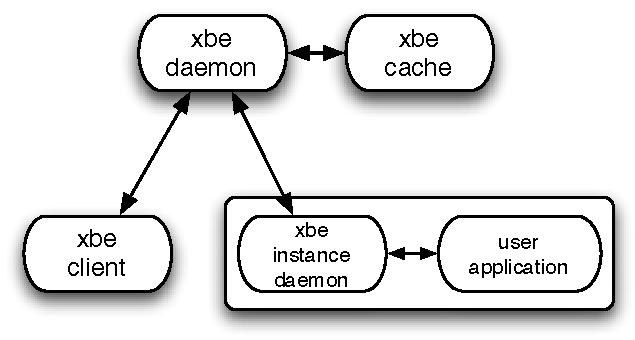
\includegraphics[scale=.7]{architecture-overview}
  \caption[Overview of the  \gls{glo:XenBEE} components]{The components of
    the Xen-based Execution Environment}
  \label{fig:architecture-overview}
\end{figure}

On the left hand side of the picture are the users using the \emph{xbe} to
communicate with the execution  environment. The \emph{xbe} refers in this
case  to the command  line tool  which I  have implemented  as a  proof of
concept  to interact  with the  \emph{xbed}.  The  interface that  an user
utilizes to execute his applications  with the \gls{glo:XenBEE} could be a
web-portal or some other tool with a graphical user interface, as well.

\medskip

On the right hand side are the components that are required to execute the
applications within  virtual machines.  The \emph{xbed} has  to be running
on a machine, that supports  the Xen hypervisor.  It maintains an internal
connection to  a local  cache, which can  be used  by any user  to deposit
arbitrary data on the  server side.  The \emph{xbed} uses \texttt{libvirt}
to connect to the Xen hypervisor and to manage active virtual machines.

Each virtual machine  must provide the \emph{xbeinstd}, that  means it has
to be started at some point during the initialization process of the guest
operating system. Any image that is submitted to the execution environment
must therefore  contain this  program. The \emph{xbeinstd}  is responsible
for two  major issues:  executing the actual  application and  keeping the
virtual machine instance alive.   Execution of an application involves for
instance  passing  arguments  to   the  executable,  setting  the  working
directory and redirecting the input and output streams. The \emph{xbed} is
going  to shut  stale virtual  machines down,  unless  the \emph{xbeinstd}
sends  regular keep-alive  messages  to the  \emph{xbed}.   If the  user's
application has finished, the \emph{xbeinstd} signals the \emph{xbed} that
the virtual machine is ready to be shut down.

\medskip

The  thicker connections  between \emph{xbe}  and \emph{xbed}  as  well as
between \emph{xbed}  and \emph{xbeinstd} are  logical connections realized
by using message-queues and one  or more \gls{glo:MQS} in between. Whereas
he  thinner links  are either  inner-process connections  (in case  of the
cache) or  connections between  parent and child  process (in case  of the
user-application).

\section[Xen-based Execution Daemon]{Xen-based Execution Daemon (xbed)}
\label{sec:xbed}

This  section describes  the  ``heart'' of  the  \gls{glo:XenBEE} ---  the
\emph{xbed}.  Well, the \emph{xbed}  is itself composed of several smaller
components that  are each responsible for  a single detail  of the daemon.
The    main    components    though    are   the    \texttt{Cache},    the
\texttt{TaskManager}  and the  \texttt{InstanceManager}. The  former  is a
rather simple implementation of a local data cache, that will be discussed
in a later section.

\begin{figure}[ht]
  \centering
  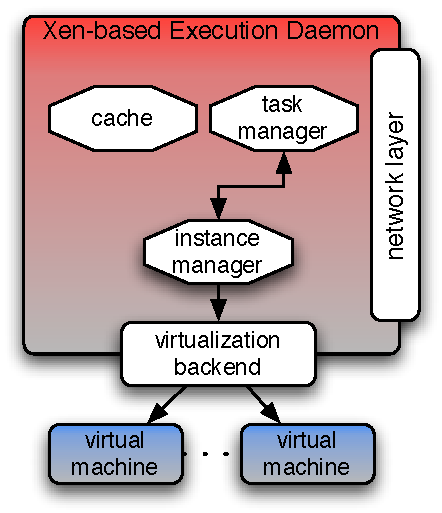
\includegraphics[scale=.55]{xbed-architecture}
  \caption[Components of the xbed]{The most important components of the xbed}
  \label{fig:xbed-architecture}
\end{figure}

\subsubsection{Network Layer}

On startup, the  daemon tries to connect to  the message-queue server that
has been  defined either in  its configuration file  or as a  command line
parameter. This process  is realized by the \emph{network  layer}. It uses
the  \texttt{twisted} framework to  establish a  \gls{glo:TCP} connection.
When the connection has been successfully established, a special transport
protocol --- the  STOMP protocol --- is attached  to the connection. STOMP
is  the \emph{Streaming  Text Oriented  Messaging Protocol}  and basically
defines a  very simple protocol to  send and receive text  messages over a
message-queue server.  On top of  this text message based protocol are XML
based  protocols  that  accomplish  the whole  communication  between  all
components.   There is currently  a basic  XML protocol  that encapsulates
single ``messages'', consisting just of header and body, and two protocols
that  connect up  the \emph{xbe}  and the  \emph{xbeinst}  accordingly.  A
special  protocol providing  security related  services  (i.e.~privacy and
validity) can be added as an additional layer.

Anyway, the  details of the \gls{glo:STOMP}  and XML protocols  as well as
the network layer,  which is to some extent equal  among all components of
the        \gls{glo:XenBEE},       will       be        discussed       in
Section~\ref{sec:communication-protocol},
\emph{\nameref{sec:communication-protocol}}.

\subsubsection{Task-Manager}

When an  user submits,  terminates or  requests the status  of one  of her
jobs, the  message is actually handled by  the \texttt{TaskManager}.  This
component controls all tasks, the system knows of. A ``task'' does in this
case  not refer  to the  actual application  an user  submitted, but  to a
container that holds the task's  state machine, description and probably a
reference to the virtual machine instance used for this task.

A new task gets initialized every  time an user requests a reservation. At
this time it contains nothing more  than the state machine which is in its
start-state                               (i.e.~\texttt{Pending:Reserved}).
Section~\ref{sec:xbed:job-model}  discusses   the  implementation  of  the
job-model that has been used to  represent an activity.

Each task and each reservation has its own unique identifier by which they
are known  to the system  and to the  user.  Those unique  identifiers are
implemented     by    using     \emph{Universal     Unique    Identifiers}
(\gls{glo:UUID}s).  Whereas  the task identifier is more  or less publicly
available\footnote{a listing  of all current tasks comparable  to the UNIX
  \texttt{ps}  command could be  possible}, the  identifier of  the user's
reservation is  only known to  that particular user (or  some intermediary
software such as  a Calana-agent). All requests that an  user makes to the
system,  that refer  to a  reservation and  hence to  a task,  require the
reservation's unique identifier.

When an user confirms a reservation,  he also sends the job description as
a \gls{glo:JSDL}  document along with the confirmation  message.  The task
is  thus completely  specified and  may  perform the  transition into  the
\texttt{Executing} state. To this time, the task-manager creates a special
spool directory  for that  task which is  eventually going to  contain all
necessary  files to  create the  virtual  machine and  execute the  user's
application. The  details of how the  required files are  obtained will be
discussed  in   a  later  section  (Section~\ref{sec:xbed:data-transfer}).
After  all   files  have  been   retrieved,  the  \texttt{InstanceManager}
component is used to create a new virtual machine for the task.

\subsubsection{Instance-Manager}

The instance-manager's purpose is  to create, control, monitor and destroy
active virtual  machine instances.  Again  unique identifiers are  used to
name the  virtual machines. To start  a virtual machine  several files are
required:  an   operating  system  installation  residing   in  a  special
file-system \gls{glo:image} file, a \gls{glo:kernel}

\begin{itemize}
\item uuid usage in several places
\item task manager
\item instance manager
\item ticket store
\item back-end (currently only implemented for xen)
\item networking layer
\item cache
\end{itemize}

\subsection{Job-model Implementation}
\label{sec:xbed:job-model}

The  task-manager not only  manages and  creates tasks,  but also  holds a
queue of current activities of each task.


\begin{itemize}
\item activity queue (picture)
\item threads
\end{itemize}

\begin{figure}[ht]
  \centering
  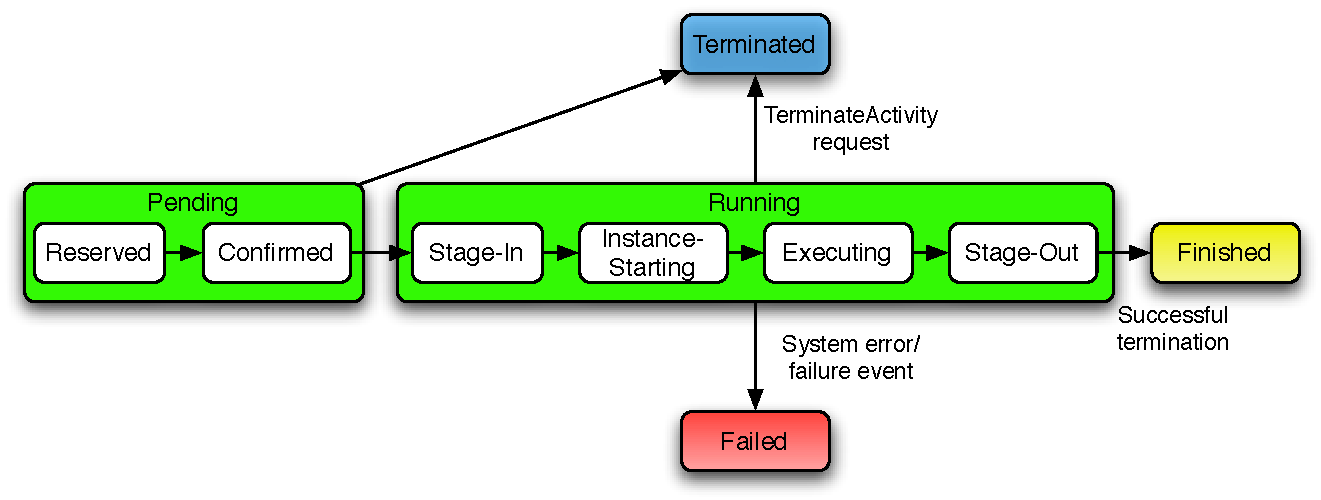
\includegraphics[scale=.55]{bes-job-model}
  \caption{The job-model used in the \gls{glo:XenBEE}}
  \label{fig:bes-extended-xen}
\end{figure}

\begin{figure}[ht]
  \centering
  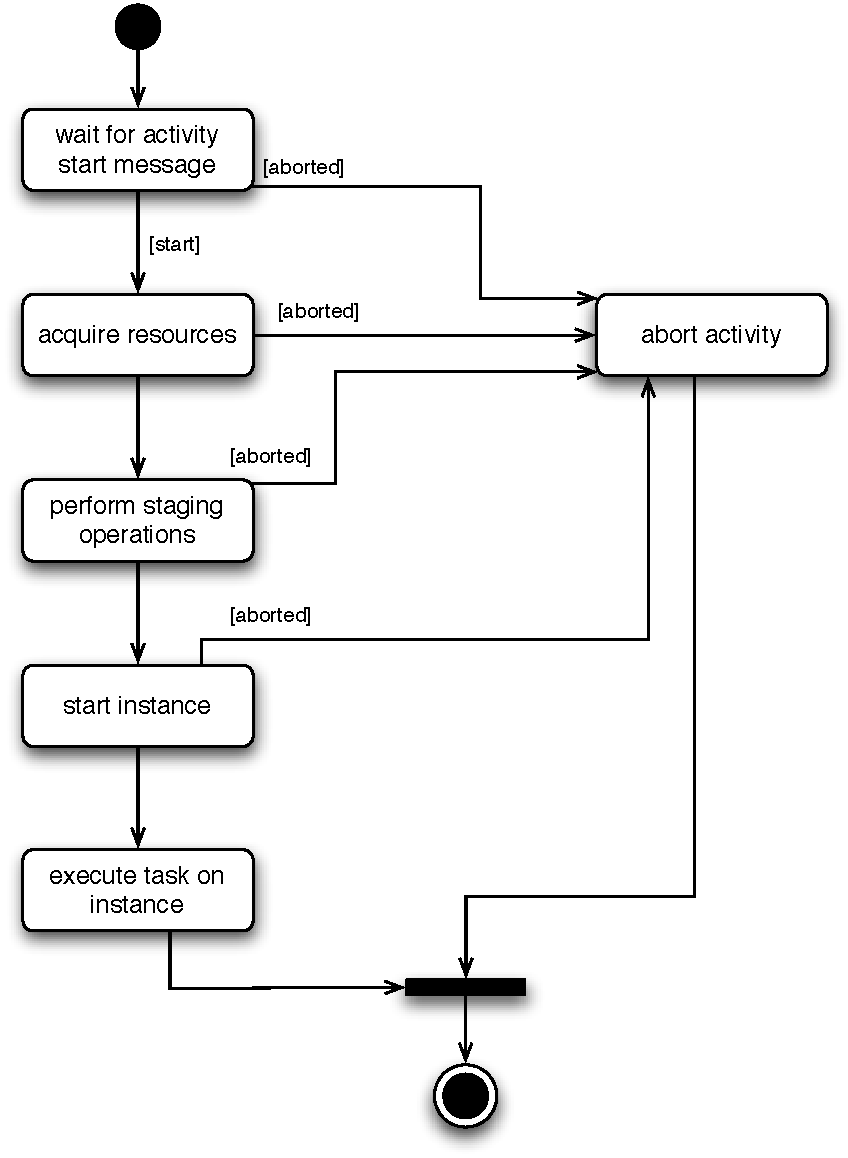
\includegraphics[scale=.55]{act-start-task}
  \caption[Start Task Activity]{TODO: fill me in}
  \label{fig:act-start-task}
\end{figure}

\begin{figure}[ht]
  \centering
  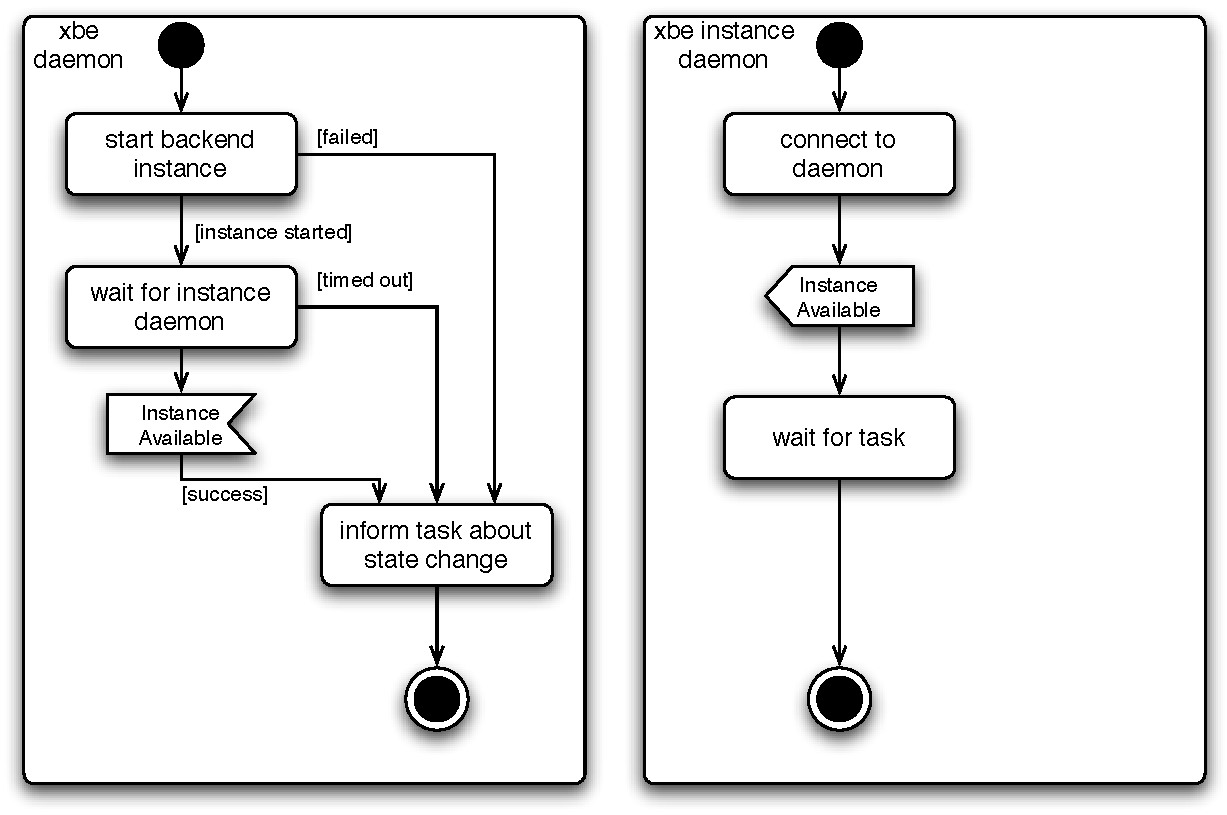
\includegraphics[scale=.55]{act-start-instance}
  \caption[Start Instance Activity]{TODO: fill me in}
  \label{fig:act-start-instance}
\end{figure}


\subsection{Data Transfer Handling}
\label{sec:xbed:data-transfer}

\begin{itemize}
\item uri
\item cache references
\item failure
\item validation (hashes)
\item compression
\item user interaction --- terminate
\end{itemize}

\begin{figure}[ht]
  \centering
  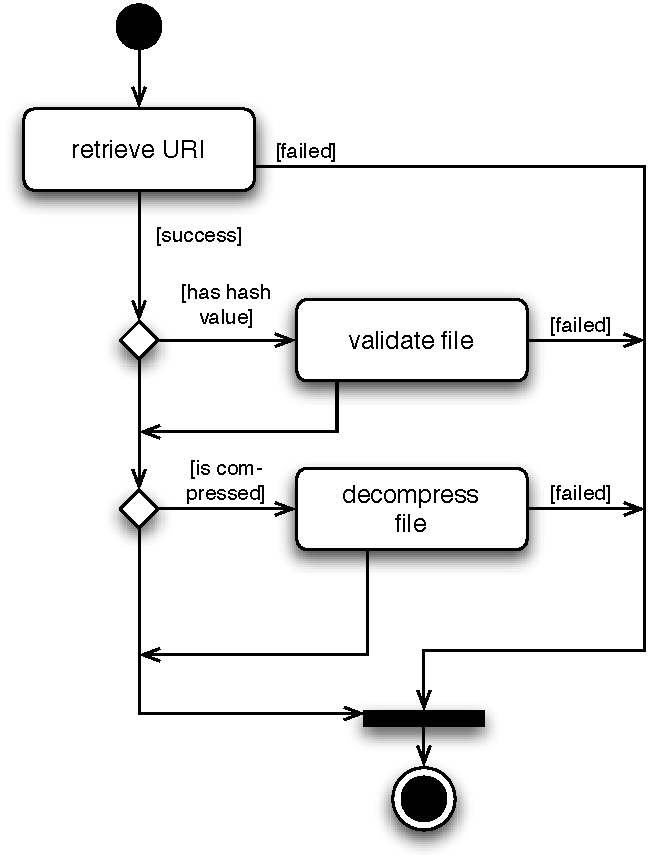
\includegraphics[scale=.7]{act-retrieve-file}
  \caption[File Retrieval Activity]{TODO: fill me in}
  \label{fig:act-retrieve-file}
\end{figure}


\begin{figure}[ht]
  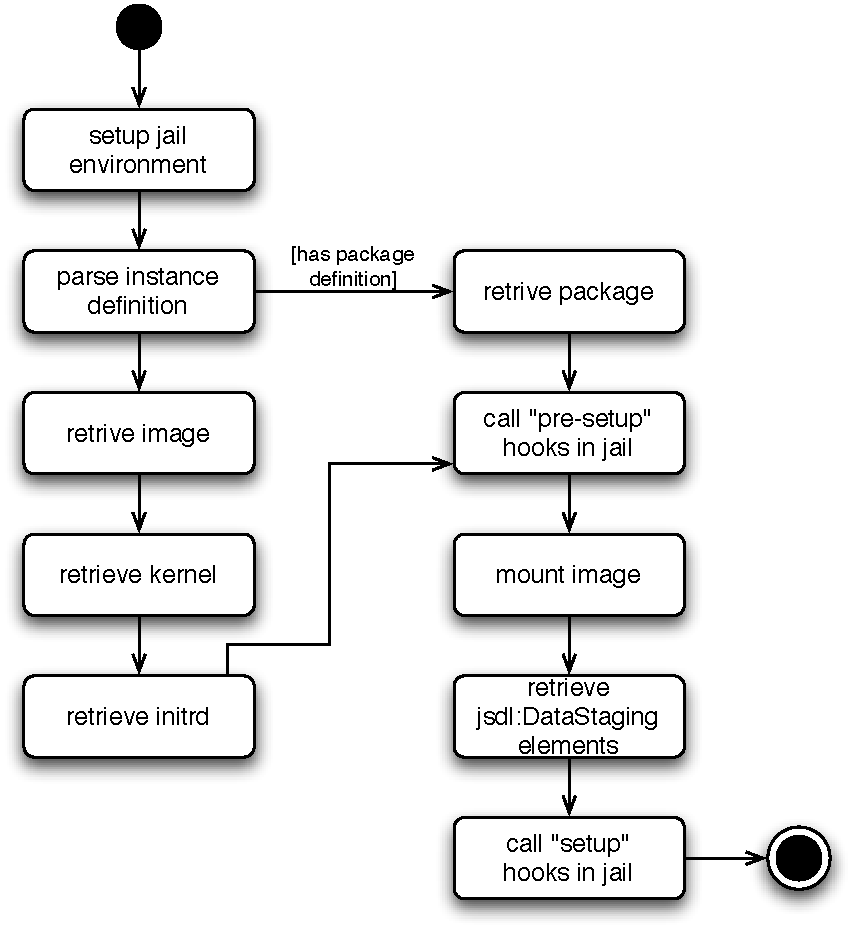
\includegraphics[scale=.7]{act-stage-in}
  \caption[Stage-In Activity]{TODO: fill me in}
  \label{fig:act-stage-in}
\end{figure}


\subsection{Caching Of Arbitrary Files}
\label{sec:caching}

\begin{itemize}
\item addToCache
\item uri based retrieval
\item uuid as cache entry id
\item referencing to entries
\item description for cached data
\item data types (image, kernel, initrd, data)
\item database
\end{itemize}

\subsubsection{Adding data to the cache}

\subsubsection{Discovering cache entries}

\begin{figure}[ht]
  \centering
  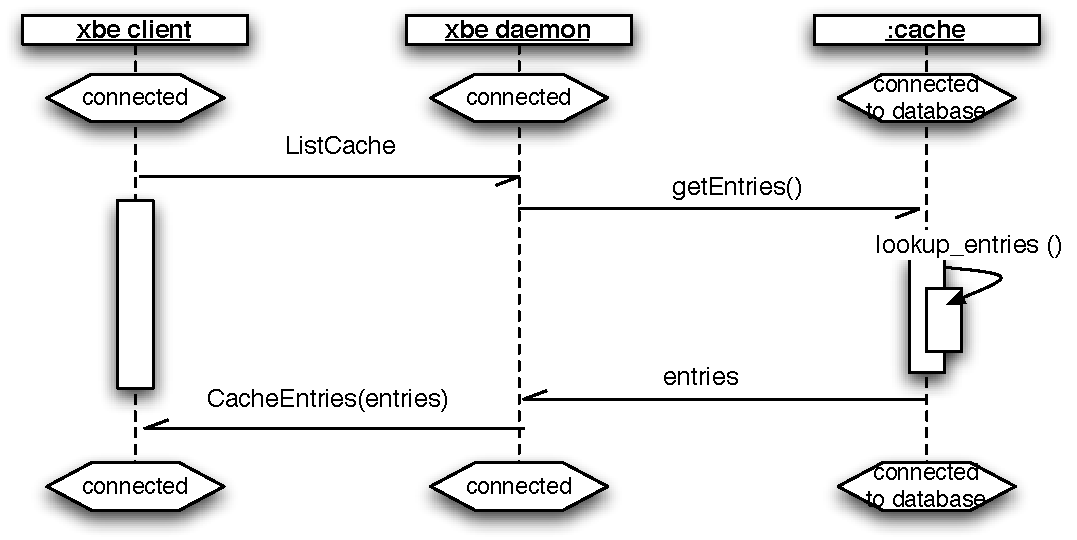
\includegraphics[scale=.75]{msc-list-cache}
  \caption[MSC List Cache Entries]{TODO: fill me in}
  \label{fig:msc-list-cache}
\end{figure}

\subsubsection{Using cache entries}

\subsection{Instance Configuration}

\section[Xen-based Execution Instance Daemon]{Xen-based Execution Instance Daemon (xbeinstd)}
\label{sec:xbeinstd}

\begin{itemize}
\item notifies xbed when instance is up (i.e. network connectivity)
\item keep-alive
\item input files are already available
\item parses jsdl
\item sets working directory
\item redirects standard input/output/error to the files in jsdl (or /dev/null)
\item starts task when the xbed notifies
\item passes arguments specified in jsdl
\item notifies xbed when application has finished (shutdown may be initialized)
\end{itemize}
foo bar

\section{The Communication Protocol}
\label{sec:communication-protocol}

\begin{itemize}
\item make reservation
\item confirm reservation (jsdl) +/- start
\item submit whole job (make res + confirm)
\item terminate activity
\item status request
\item add cache entry
\item security establishment (certificates, encryption, signing)
\item stomp
\end{itemize}

\subsection{STOMP}
\label{sec:protocol:stomp}

\subsection{MSCs}

\begin{figure}[ht]
  \centering
  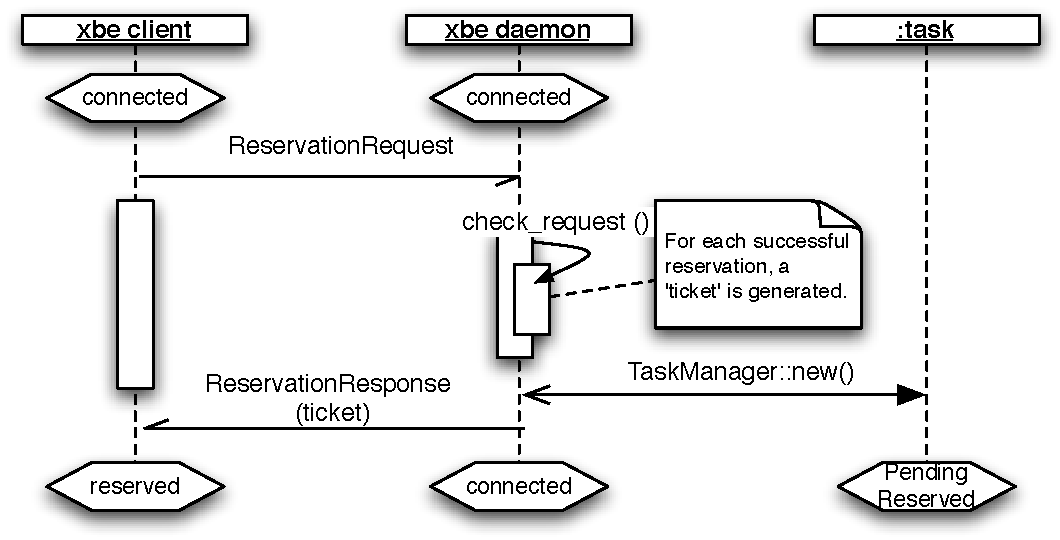
\includegraphics[scale=.75]{msc-reserve}
  \caption[MSC Make Reservation]{TODO: fill me in}
  \label{fig:msc-reserve}
\end{figure}

\begin{figure}[ht]
  \centering
  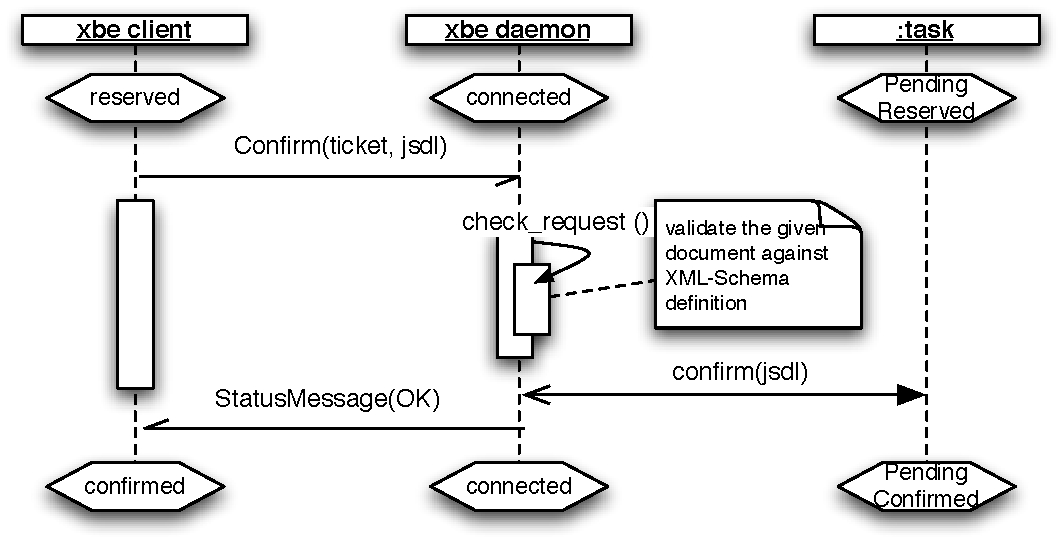
\includegraphics[scale=.75]{msc-confirm}
  \caption[MSC Confirm Reservation]{TODO: fill me in}
  \label{fig:msc-confirm}
\end{figure}

\begin{figure}[ht]
  \centering
  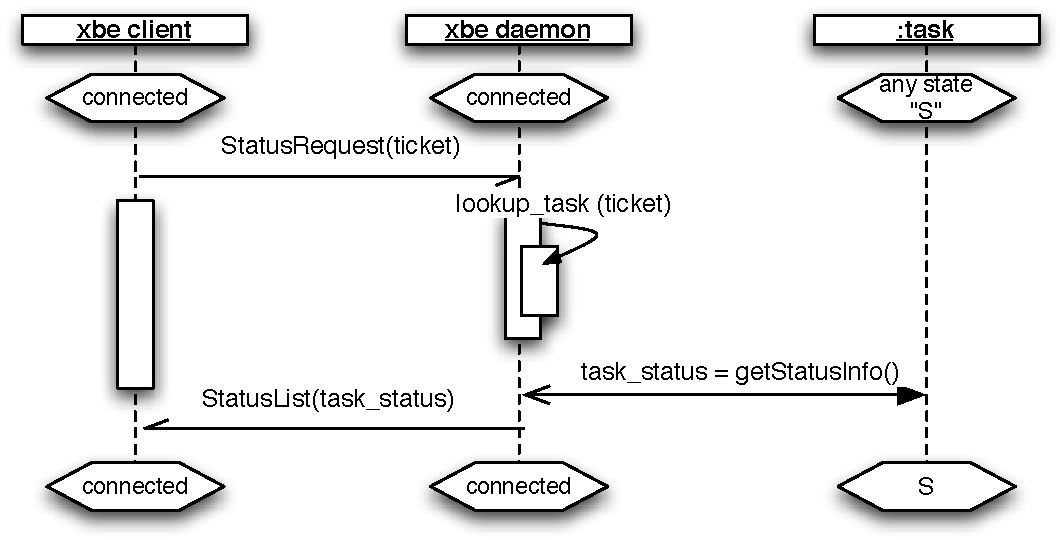
\includegraphics[scale=.75]{msc-status-request}
  \caption[MSC Request Task Status]{TODO: fill me in}
  \label{fig:msc-status-request}
\end{figure}

\begin{figure}[ht]
  \centering
  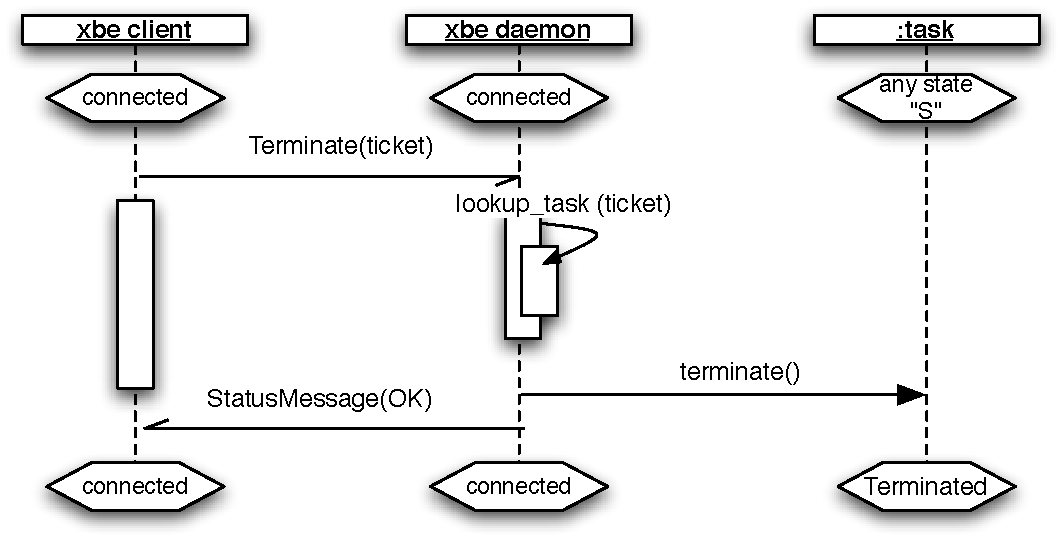
\includegraphics[scale=.75]{msc-terminate}
  \caption[MSC Terminate Task Request]{TODO: fill me in}
  \label{fig:msc-terminate}
\end{figure}

\subsection{Network Topology}
\label{sec:network-topology}

\begin{itemize}
\item simple topology: just one mqs (preferably on the xbed-host)
\item advanced topology: many mqs with configured forwarding
\item avoids common problems that arise with NAT and firewall policies
\item xbeinstd and possibly the application use the same mqs as the xbed
\end{itemize}

\begin{figure}[ht]
  \centering
  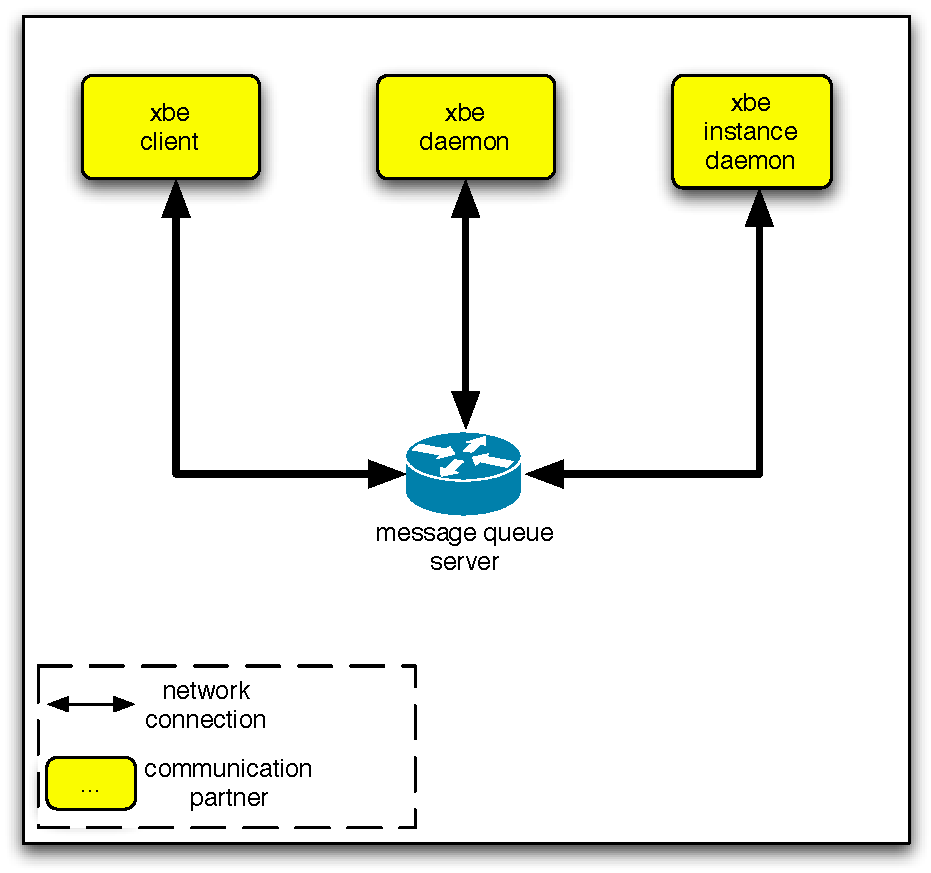
\includegraphics[scale=.75]{simple-network-topology}
  \caption[Network  Topology   (simple)]{The  simplest  network  topology,
    consisting of  only one Message  Queue Server and  three communication
    partners.}
  \label{fig:simple-net-top}
\end{figure}

\begin{figure}[ht]
  \centering
  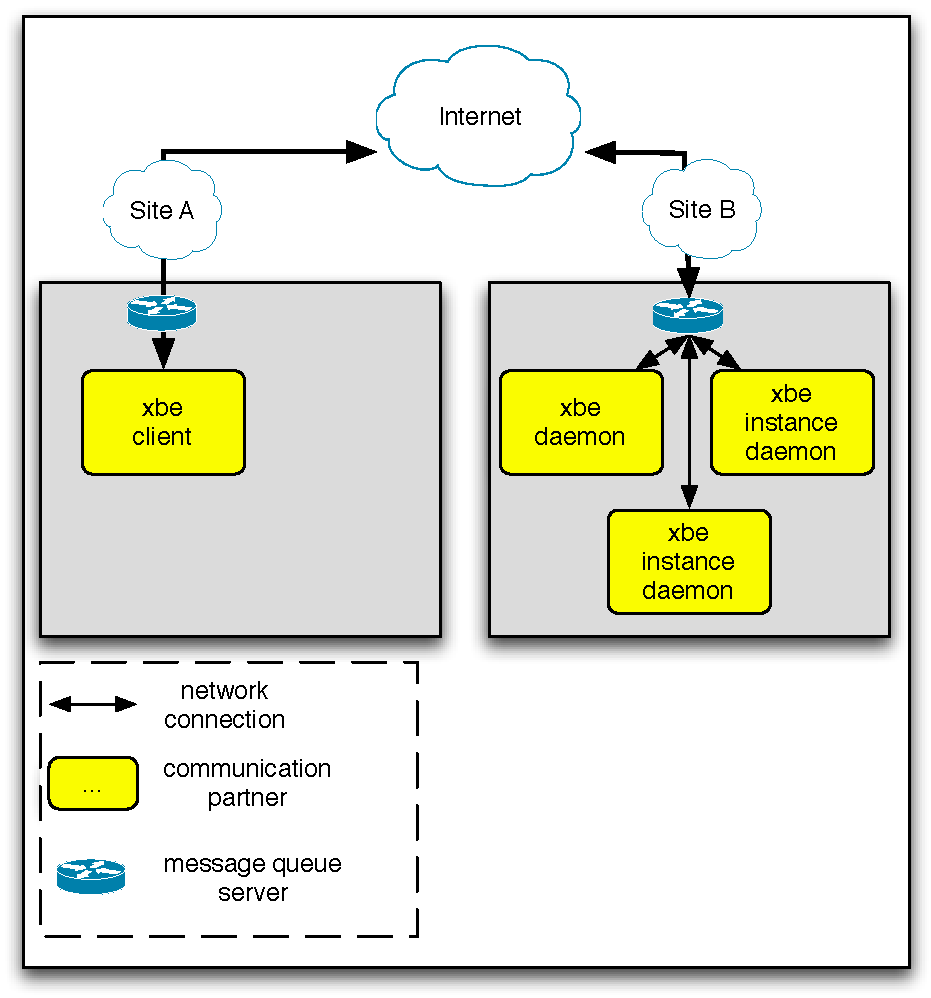
\includegraphics[scale=.75]{network-topology}
  \caption[Network  Topology]{TODO: fill me in}
  \label{fig:net-top}
\end{figure}

\subsection{Security}
\label{sec:security}

\begin{itemize}
\item symmetric encryption one-time key
\item signing of whole message
\item encryption of body
\item xml-message-security
\end{itemize}

\begin{figure}[ht]
  \centering
  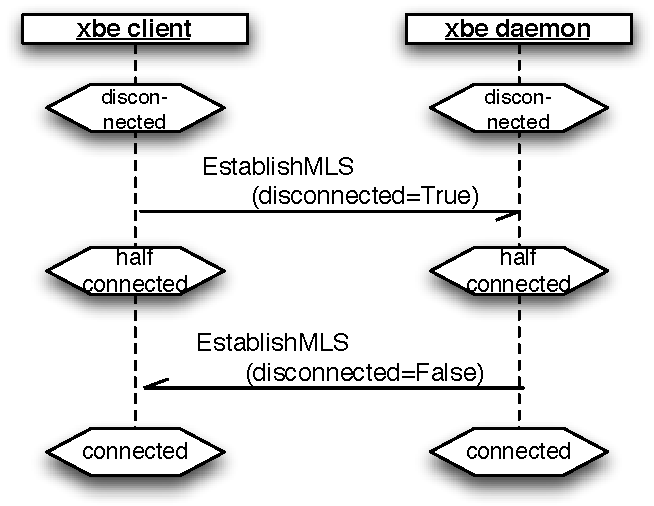
\includegraphics[scale=.75]{msc-establish-mls}
  \caption[MSC Message Layer Security]{TODO: fill me in}
  \label{fig:msc-establish-mls}
\end{figure}


\begin{figure}[ht]
  \centering
  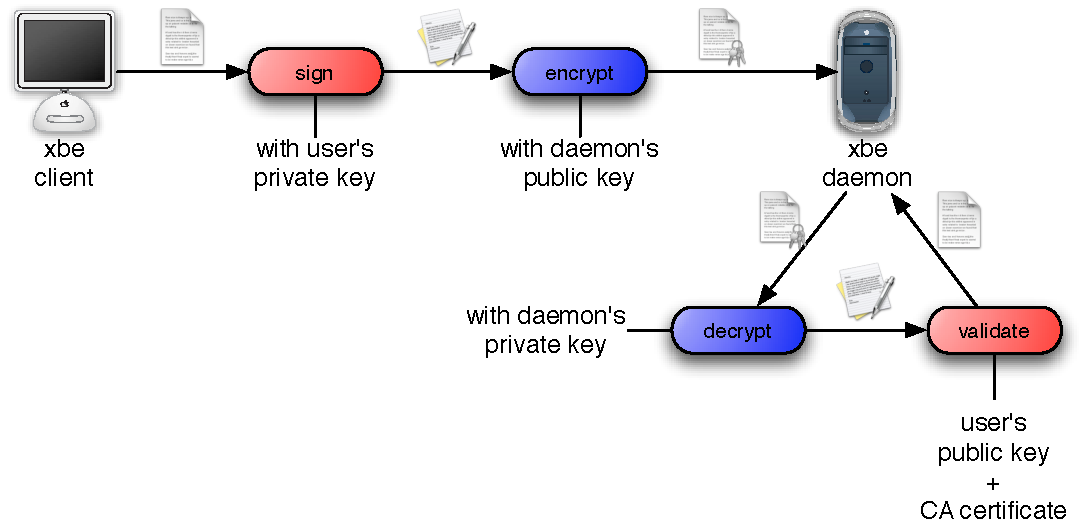
\includegraphics[scale=.75]{message-layer-security}
  \caption[Message Layer Security]{TODO: fill me in}
  \label{fig:net-mls}
\end{figure}

\subsubsection{m2crypto / openssl}

\begin{itemize}
\item problems with m2crypto on 64bit architecture
\item both are currently incompatible to each other
\item both sides (client/server) have to use the same --- eiterh m2 or
  direct openssl
\end{itemize}

%%% Local Variables: 
%%% mode: latex
%%% TeX-master: "main"
%%% End: 
